\documentclass[paper=a4, fontsize=11pt]{scrartcl} % A4 paper and 11pt font size

% ---- Entrada y salida de texto -----

\usepackage[T1]{fontenc} % Use 8-bit encoding that has 256 glyphs
\usepackage[utf8]{inputenc}
\usepackage[a4paper, total={6in, 9in}]{geometry}
%\usepackage{fourier} % Use the Adobe Utopia font for the document - comment this line to return to the LaTeX default

% ---- Idioma --------

\usepackage[spanish, es-tabla]{babel} % Selecciona el español para palabras introducidas automáticamente, p.ej. "septiembre" en la fecha y especifica que se use la palabra Tabla en vez de Cuadro

% ---- Otros paquetes ----


\usepackage{amsmath,amsfonts,amsthm} % Math packages
%\usepackage{graphics,graphicx, floatrow} %para incluir imágenes y notas en las imágenes
\usepackage{graphics,graphicx, float, url} %para incluir imágenes y colocarlas
\usepackage{eurosym}
% Para hacer tablas comlejas
%\usepackage{multirow}
%\usepackage{threeparttable}

%\usepackage{sectsty} % Allows customizing section commands
%\allsectionsfont{\centering \normalfont\scshape} % Make all sections centered, the default font and small caps

%Esto es para hipervinculos
\usepackage[hidelinks]{hyperref}

%list code
\usepackage{listings}



\usepackage{tikz}
\usetikzlibrary{positioning}
% para grafos


\hypersetup{
    colorlinks=true,
    linkcolor=blue,
    filecolor=blue,      
    urlcolor=blue,
    citecolor=blue,
    pdftitle={Overleaf Example},
    pdfpagemode=FullScreen,
    }

\urlstyle{same}
\usepackage{gensymb}
\usepackage{fancyhdr} % Custom headers and footers
\pagestyle{fancyplain} % Makes all pages in the document conform to the custom headers and footers
\fancyhead{} % No page header - if you want one, create it in the same way as the footers below
\fancyfoot[L]{} % Empty left footer
\fancyfoot[C]{} % Empty center footer
\fancyfoot[R]{\thepage} % Page numbering for right footer
\renewcommand{\headrulewidth}{0pt} % Remove header underlines
\renewcommand{\footrulewidth}{0pt} % Remove footer underlines
\setlength{\headheight}{13.6pt} % Customize the height of the header

\numberwithin{equation}{section} % Number equations within sections (i.e. 1.1, 1.2, 2.1, 2.2 instead of 1, 2, 3, 4)
\numberwithin{figure}{section} % Number figures within sections (i.e. 1.1, 1.2, 2.1, 2.2 instead of 1, 2, 3, 4)
\numberwithin{table}{section} % Number tables within sections (i.e. 1.1, 1.2, 2.1, 2.2 instead of 1, 2, 3, 4)

\setlength\parindent{0pt} % Removes all indentation from paragraphs - comment this line for an assignment with lots of text

\newcommand{\horrule}[1]{\rule{\linewidth}{#1}} % Create horizontal rule command with 1 argument of height
\usepackage{subcaption}

\title{	
\normalfont \normalsize 
\textsc{{\textbf{Aprendizaje Profundo (2024-2025)}} \\ Máster en Robótica e Inteligencia Artificial \\ Universidad de León} \\ [20pt] % Your university, school and/or department name(s)
\horrule{0.5pt} \\[0.4cm] % Thin top horizontal rule
\huge Práctica 3 \\   % The assignment title
\horrule{1.5pt} \\[0.2cm] % Thick bottom horizontal rule
}

\author{Sheila Martínez Gómez\\
Alejandro Mayorga Caro\\
Ángel Morales Romero\\
}
 % Nombre y apellidos
 % Incluye la fecha actual

\begin{document}

\maketitle
\newpage %inserta un salto de página

\tableofcontents % para generar el índice de contenidos
\pagebreak

\section{Abstract}

En este proyecto se va a realizar la siguiente tarea:

Uso de un conjunto de datos difícilmente separables para entrenar una red MLP multicapa con el objetivo de realizar la clasificación de dichos datos. 

Una vez entrenada se visualizarán los datos a la salida de cada una de las capas, aportando la interpretación de la transformación efectuada por dicha capa. 

El objetivo es reconocer las distintas transformaciones que las capas van aplicando a los datos de partida hasta convertirlos en linealmente separables.

\section{Estudio del dataset}

El dataset escogido es el \textit{Moons Dataset}, que se obtiene de \textbf{Sklearn}. Es un dataset difícilmente separable, que contiene datos que forman dos semicírculos o lunas que no se superponen. Es un dataset utilizado normalmente para visualizar \textit{clustering} y trabajar con algoritmos de clasificación. 

En este caso se ha inicializado con los siguientes valores:
\begin{itemize}
    \item \textbf{n\_samples}: 2000
    \item \textbf{noise}: 0.25
    \item \textbf{random\_state}: 0
\end{itemize}

Si bien es importante recalcar que el valor \textbf{random\_state} no tiene ningún efecto muy significativo, pues únicamente sirve para asegurar la replicabilidad de las pruebas que se realizan. 

\begin{figure}[H]
\caption{Representación del conjunto \textit{moons dataset}}
\centering
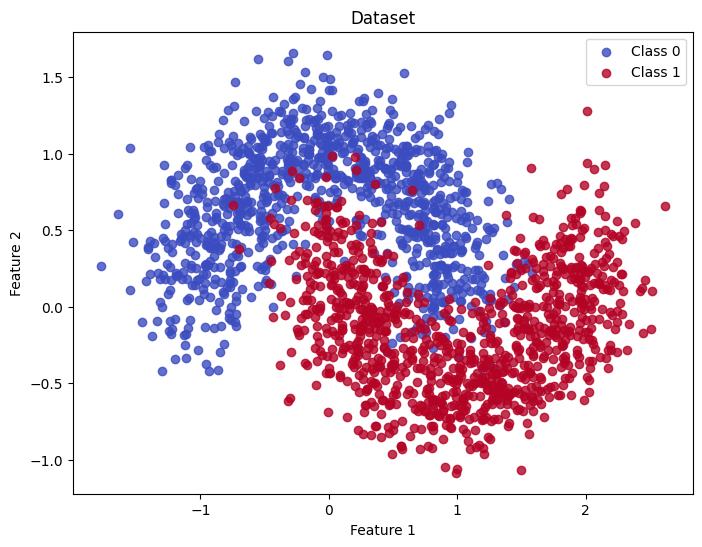
\includegraphics[width=0.5\textwidth]{images/moons_plot.png}
\end{figure}

Como puede verse, este conjunto no puede separarse de manera precisa mediante un clasificador lineal, por lo que cumple a la perfección los requisitos de la tarea.

Consta de dos clases, que llamaremos \textbf{Clase 0} y \textbf{Clase 1}. 

\begin{verbatim}
import numpy as np
import matplotlib.pyplot as plt
from sklearn.datasets import make_moons

# Number of samples
n_samples = 2000

# Generate the dataset
X, y = make_moons(n_samples=n_samples, noise=0.25, random_state=0)
\end{verbatim}

\section{Clasificación}
\subsection{Preprocesamiento}

Para comenzar a trabajar con este dataset se debe realizar una división del conjunto en tres grupos de datos, \textbf{entrenamiento}, \textbf{validación} y \textbf{test}. Se ha escogido la siguiente distribución:

\begin{itemize}
    \item \textbf{Entrenamiento}: 64\% del conjunto.
    \item \textbf{Validación}: 16\% del conjunto.
    \item \textbf{Test}: 20\% del conjunto.
\end{itemize}

\begin{verbatim}
    
xtrn, xtst, ytrn, ytst = train_test_split(X, y, test_size=0.2, random_state=seed)
xtrn, xval, ytrn, yval = train_test_split(xtrn, ytrn, test_size=0.2, random_state=seed)
\end{verbatim}

Si imprimimos el argumento \textit{shape} de cada set, podremos confirmar que el conjunto se ha separado correctamente:

\begin{verbatim}
Training set shape: (1280, 2) (1280,)
Validation set shape: (320, 2) (320,)
Test set shape: (400, 2) (400,)

\end{verbatim}

Si mostramos uno de los sets podremos confirmar que los datos que se han extraído siguen estando generalizados con respecto al conjunto inicial:

\begin{figure}[H]
\caption{Representación del conjunto de test generado}
\centering
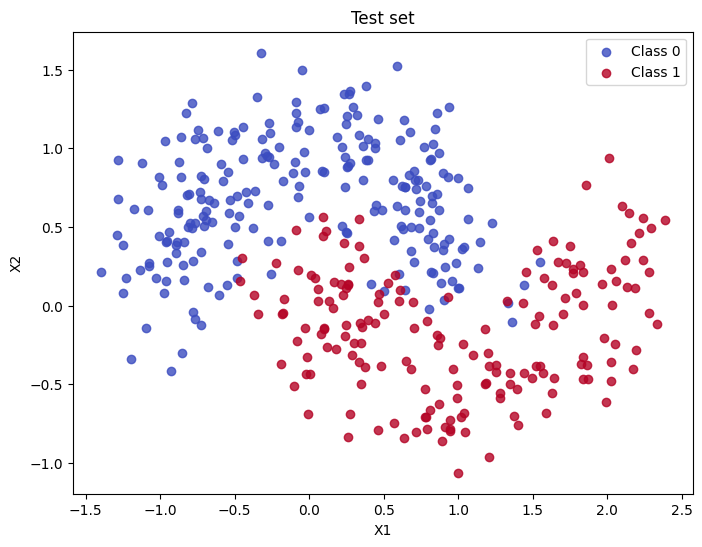
\includegraphics[width=0.5\textwidth]{images/test_output.png}
\end{figure}

\subsection{Creación de la red neuronal}

Para realizar la división del conjunto se utilizará una red neuronal con modelo \textbf{secuencial}. Constará de las capas propuestas a continuación:

\begin{figure}[H]
\caption{Representación de la red neuronal escogida}
\centering
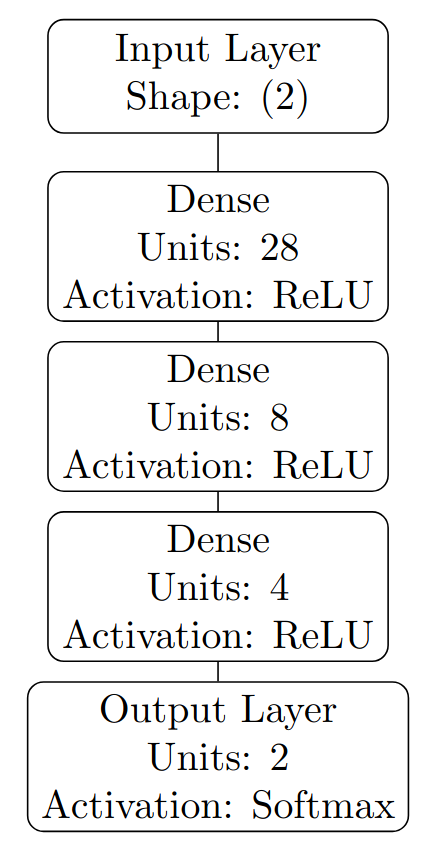
\includegraphics[width=0.3\textwidth]{images/graph.png}
\end{figure}

También se utilizará un valor de \textbf{\textit{learning rate}} de 0.001 para conseguir que el modelo aprenda de manera estable y el modelo converja más rápidamente.

\begin{verbatim}
# Create the MLP
model = Sequential()

input_layer = Input(shape=(2,), name='input_layer')
layer1 = Dense(28, activation='relu', name='layer1')(input_layer)
layer2 = Dense(8, activation='relu', name='layer2')(layer1)
layer3 = Dense(4, activation='relu', name='layer3')(layer2)
output_layer = Dense(2, activation='softmax', name='output_layer')(layer3)

model = Model(inputs=input_layer, outputs=output_layer)

# Compile the model
optimizer = Adam(learning_rate=0.001)
model.compile(optimizer=optimizer, loss='sparse_categorical_crossentropy', metrics=['accuracy'])

\end{verbatim}

Si imprimimos el resumen del modelo obtendremos el número de parámetros y la forma que tiene cada una de las capas:

\begin{table}[H]
    \centering
    \begin{tabular}{@{}|l|c|c|@{}}
        \hline
        \textbf{Layer (type)} & \textbf{Output Shape} & \textbf{Param \#} \\ \hline
        \texttt{input\_layer (InputLayer)} & \texttt{(None, 2)} & 0 \\ \hline
        \texttt{layer1 (Dense)} & \texttt{(None, 28)} & 84 \\ \hline
        \texttt{layer2 (Dense)} & \texttt{(None, 8)} & 232 \\ \hline
        \texttt{layer3 (Dense)} & \texttt{(None, 4)} & 36 \\ \hline
        \texttt{output\_layer (Dense)} & \texttt{(None, 2)} & 10 \\ \hline
    \end{tabular}
    \caption{Resumen de la red neuronal}
    \label{tab:network_summary}
\end{table}


\subsection{Entrenamiento de la red neuronal}

Para entrenar la red neuronal y adaptarse al hardware utilizado, se dividirá el conjunto para obtener un \textit{batch-size} de cinco grupos.

Posteriormente, se entrenará el modelo durante 220 épocas.

\begin{verbatim}
# Train the model
bs = xtrn.shape[0]//5
history = model.fit(xtrn, ytrn, epochs=220, batch_size=bs, validation_data=(xval, yval))
\end{verbatim}

Una vez entrenado, y para obtener los valores que realmente son relevantes, evaluamos el modelo en el conjunto de test. Esto nos permitirá comprobar si la red generaliza bien, si se ajusta demasiado a los datos (\textit{overfitting}), o si no es suficientemente potente y no se ajusta lo necesario (\textit{underfitting}).

\begin{verbatim}
    test_loss, test_accuracy = model.evaluate(xtst, ytst)  # xtst y ytst son los datos de prueba
\end{verbatim}

Si imprimimos las curvas de progreso de \textit{accuracy} y \textit{loss}, vemos que el modelo está bien ajustado, que converge correctamente, y que no sufre de \textit{underfitting} u \textit{overfitting}.


\begin{figure}[H]
  \centering
  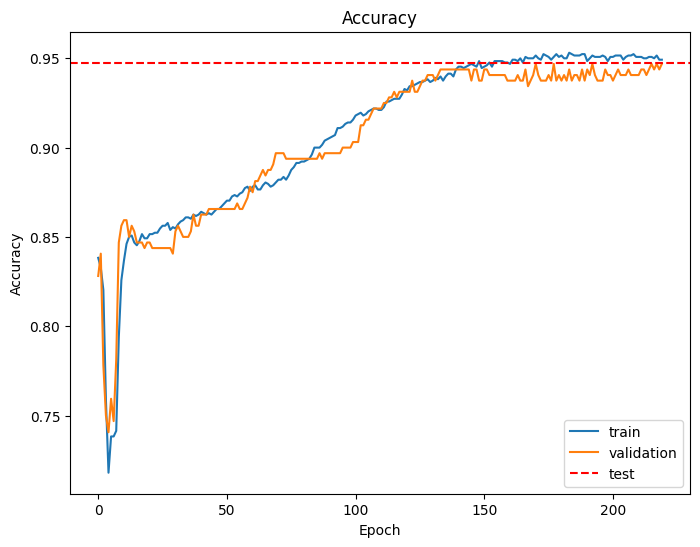
\includegraphics[width=.6\linewidth]{images/accuracy_output.png}
  \caption{\textit{Accuracy} en el set de test}
  \label{fig:sub1}
\end{figure}

\begin{figure}[H]
  \centering
  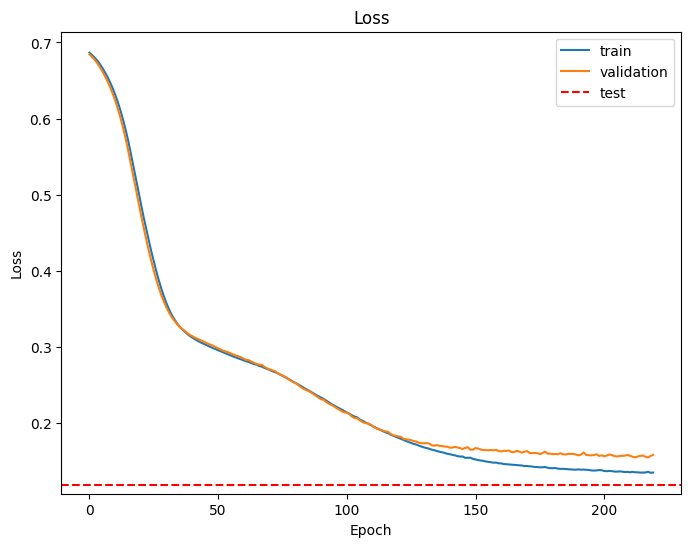
\includegraphics[width=.6\linewidth]{images/loss_output.png}
  \caption{Pérdida en el set de test}
  \label{fig:sub2}
\end{figure}

Además, el modelo obtiene una precisión de 0.9495, un valor que puede considerarse válido en esta situación. 

\subsection{Estudio capa a capa}

En esta sección se tratarán las diferentes transformaciones que aplican las neuronas en cada capa del modelo para separar los dos conjuntos del set. 


La red neuronal analizada tiene cinco capas que cumplen funciones específicas y transforman los datos para lograr una representación abstracta que facilite la clasificación.
\newpage

\subsubsection{Input Layer (\texttt{input\_layer})}
La capa de entrada tiene una forma de \texttt{(None, 2)}, lo que significa que recibe datos de entrada con dos características (\textit{Feature 1} y \textit{Feature 2}). Esta capa no realiza transformaciones y simplemente pasa los datos a la siguiente capa.


\subsubsection{Primera Capa Densa (\texttt{layer1})}
La primera capa densa contiene 28 neuronas y utiliza la función de activación ReLU (\( \text{ReLU}(x) = \max(0, x) \)). Su propósito es aprender combinaciones lineales de las características de entrada y agregar no linealidad al modelo. Esto amplía el espacio de representación de las características iniciales a 28 dimensiones, permitiendo al modelo detectar patrones más complejos.


\begin{figure}[H]
  \centering
  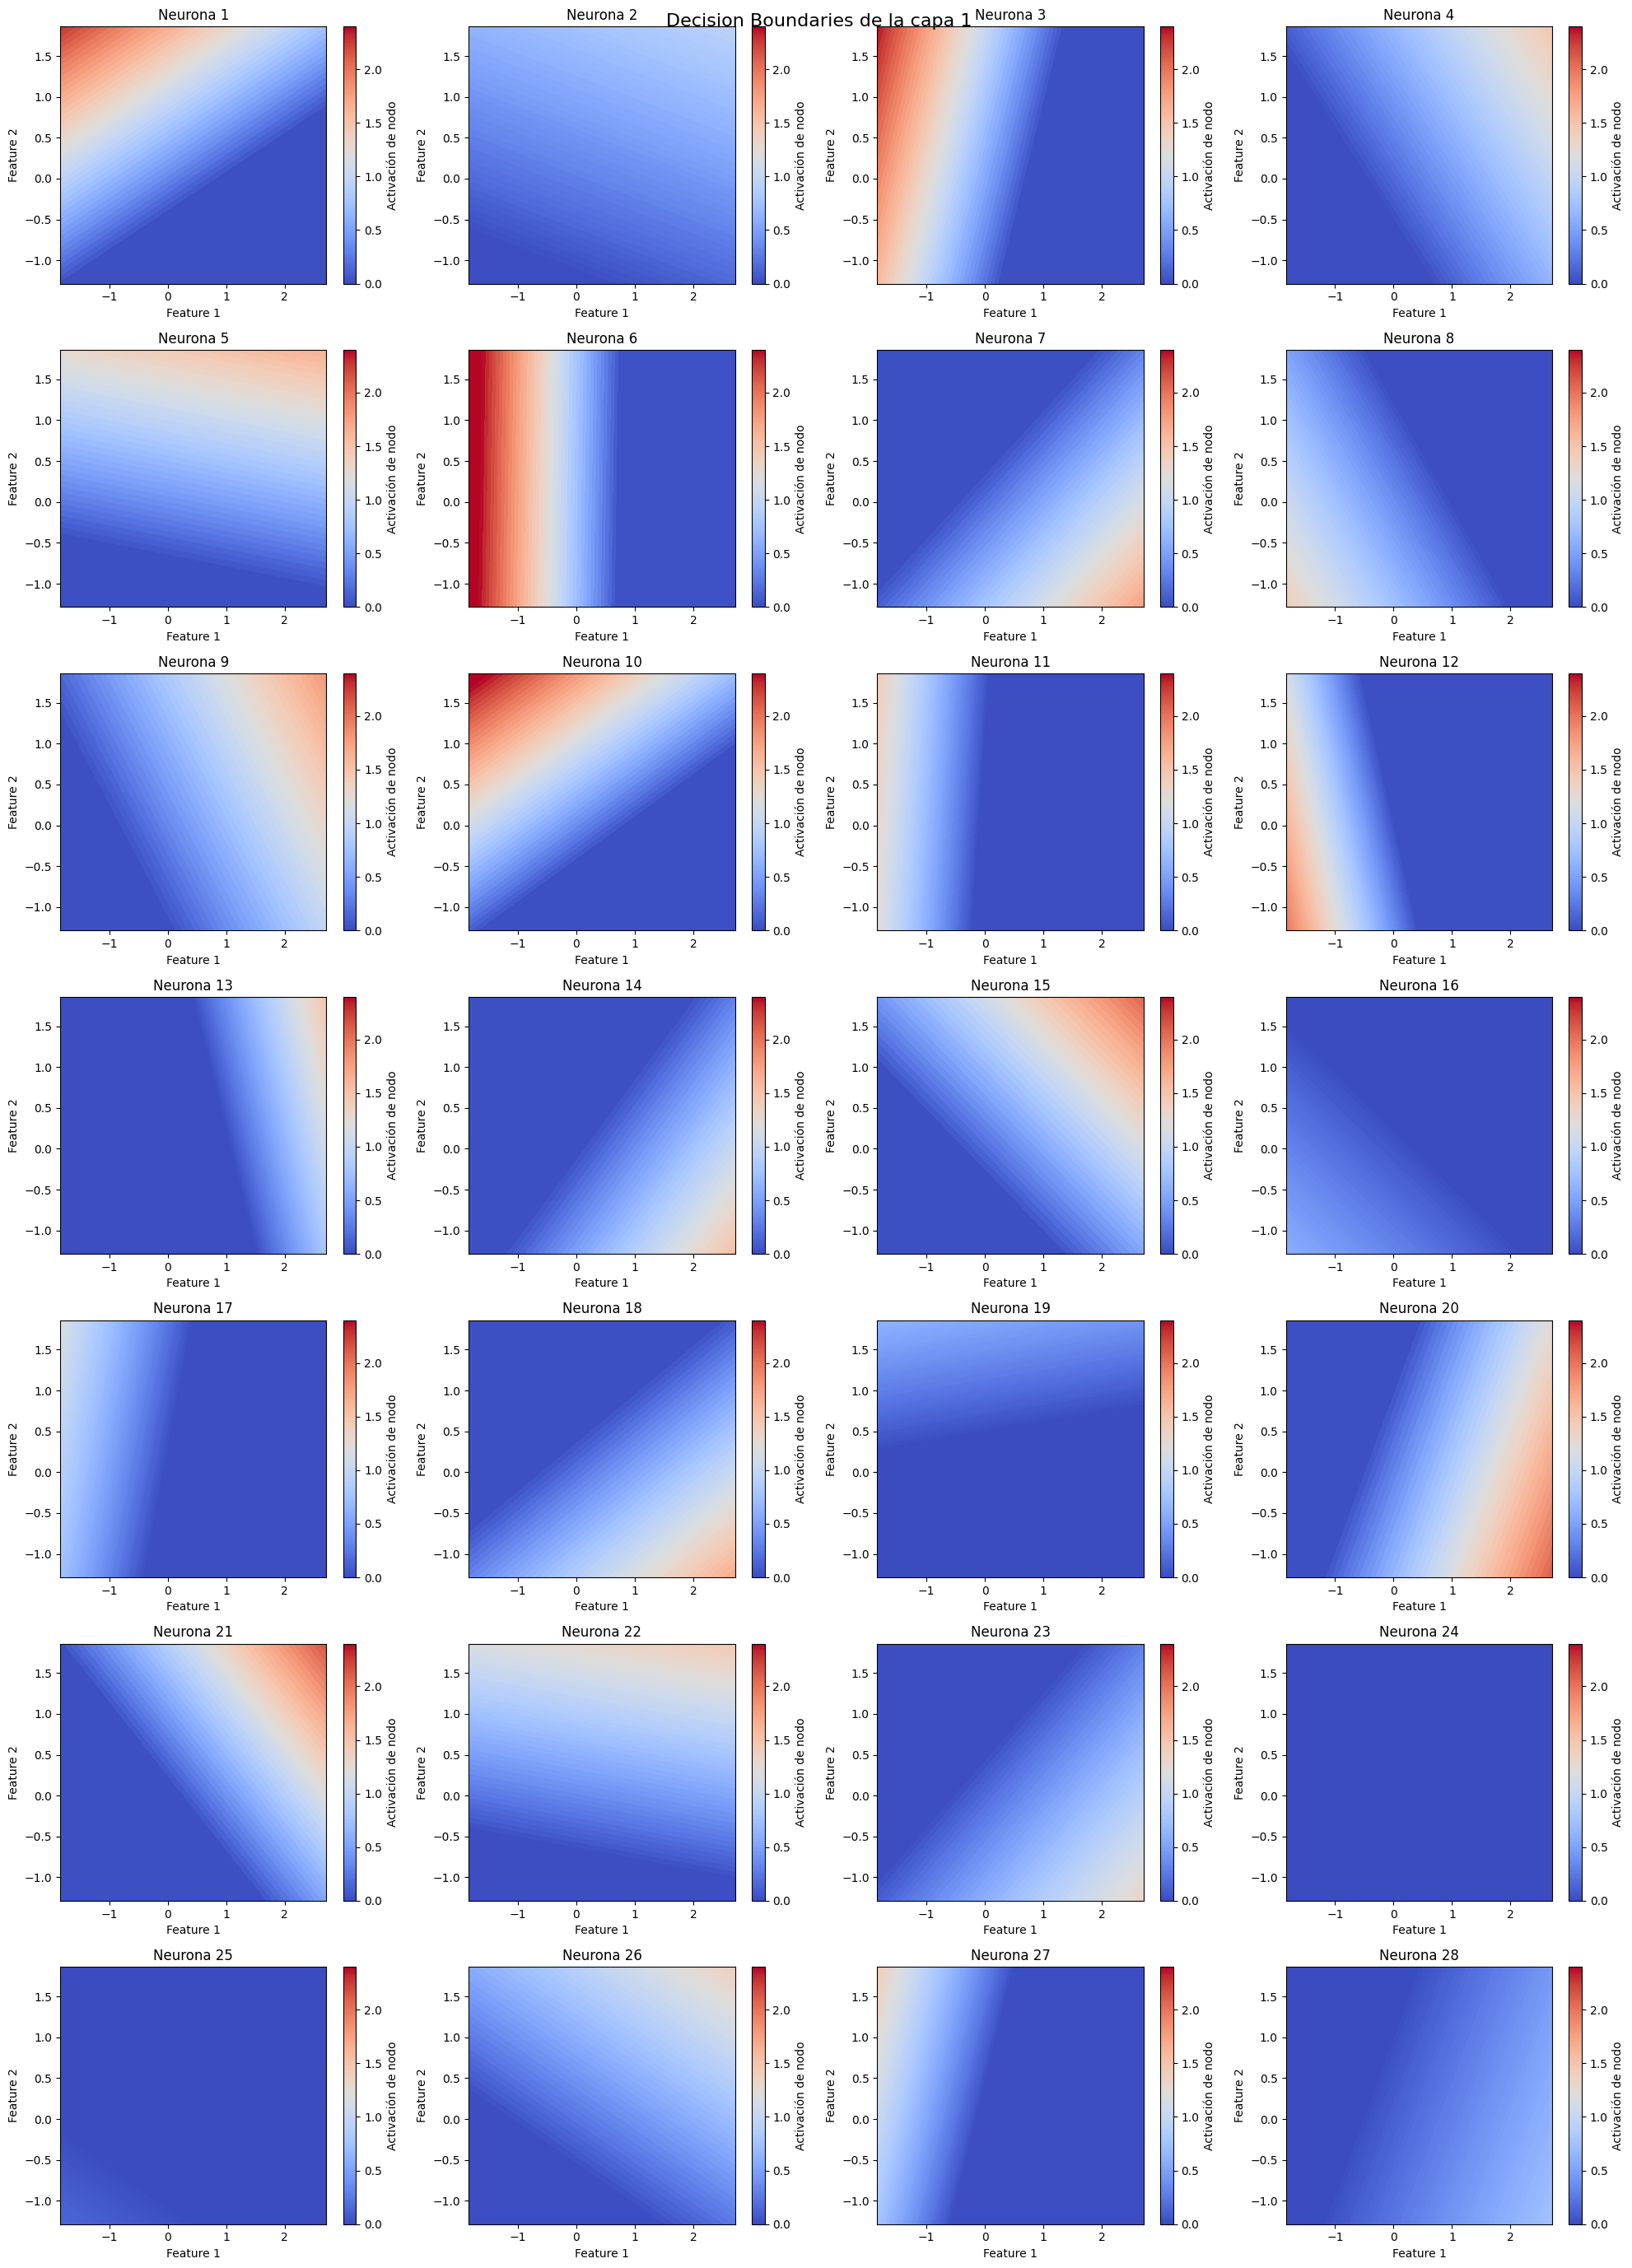
\includegraphics[width=.6\linewidth]{images/plot_neuronas_L1.png}
  \caption{Límites de decisión de las neuronas de la primera capa densa del modelo}
  \label{fig:sub1}
\end{figure}


\subsubsection{Segunda Capa Densa (\texttt{layer2})}
La segunda capa densa tiene 8 neuronas y también utiliza la función de activación ReLU. Esta capa reduce la dimensionalidad de las activaciones previas, pasando de 28 a 8 dimensiones. Las gráficas asociadas muestran cómo las activaciones de estas neuronas responden en función de las dos características de entrada. En los gráficos, las zonas rojas representan valores de activación altos, mientras que las zonas azules representan valores bajos o nulos, resultado del efecto de la función ReLU. Cada neurona en esta capa detecta patrones específicos en los datos de entrada. Algunas neuronas, como la Neurona 5, muestran activaciones planas, lo que podría indicar que tienen menor relevancia en el modelo.

\begin{figure}[H]
  \centering
  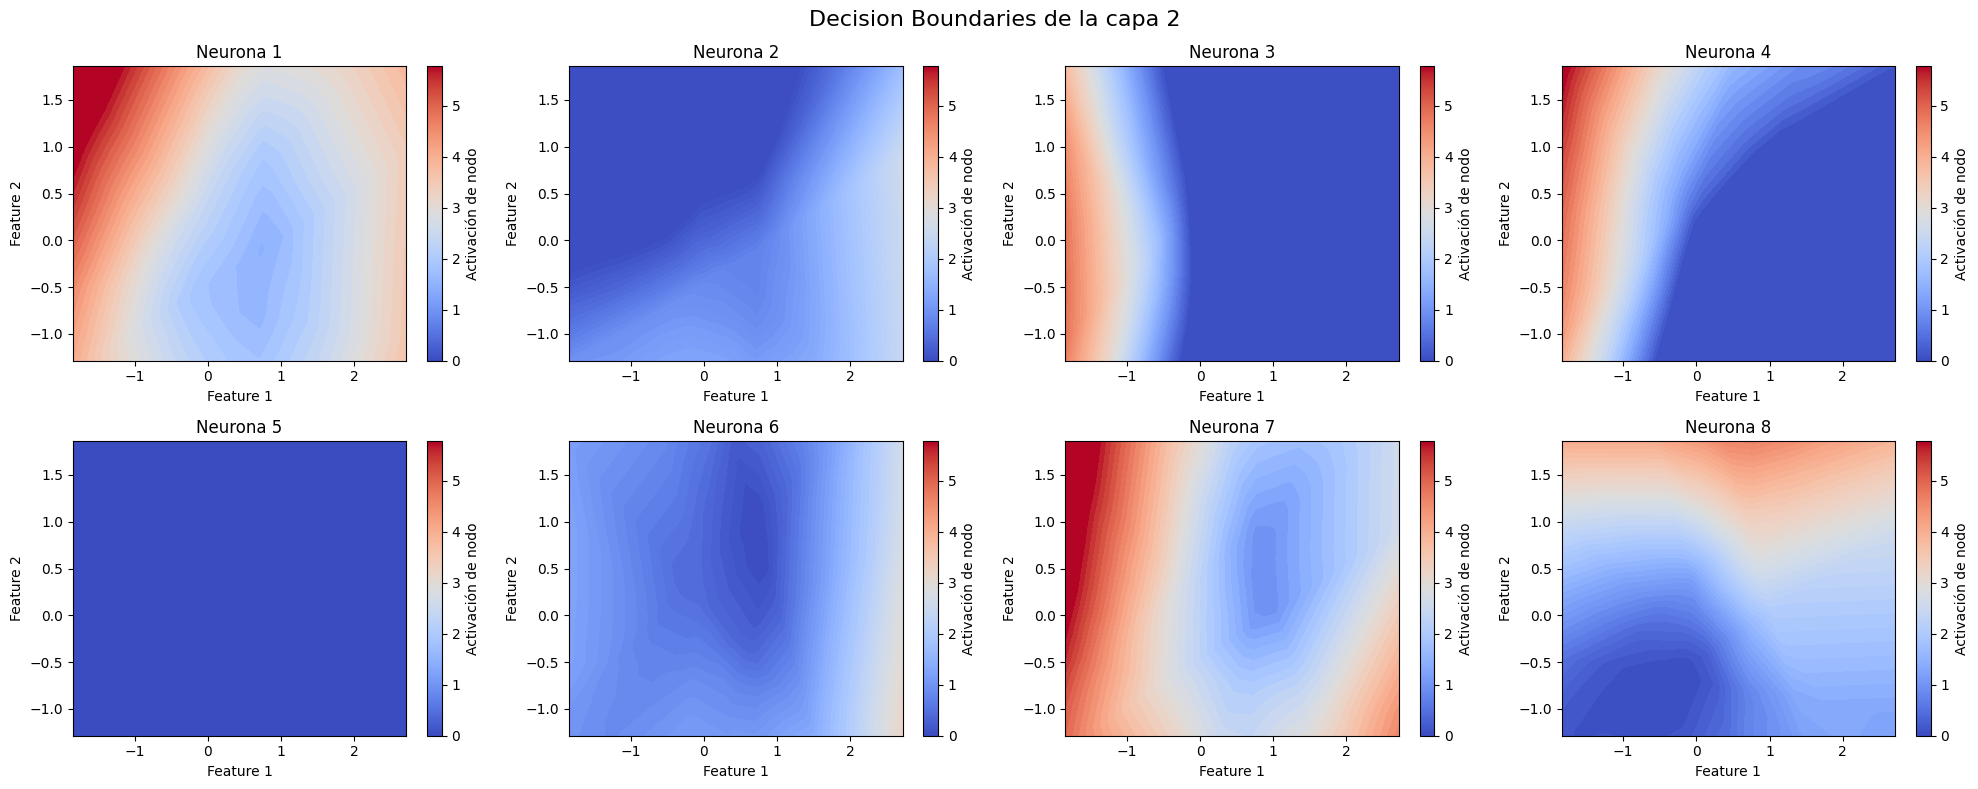
\includegraphics[width=.9\linewidth]{images/plot_neuronas_L2.png}
  \caption{Límites de decisión de las neuronas de la segunda capa densa del modelo}
  \label{fig:sub1}
\end{figure}

\subsubsection{Tercera Capa Densa (\texttt{layer3})}
La tercera capa densa tiene 4 neuronas y utiliza la función de activación ReLU. Su objetivo es reducir aún más la dimensionalidad, de 8 a 4, mientras detecta patrones más abstractos basados en las activaciones de la capa anterior. La introducción de no linealidades en esta etapa permite al modelo crear representaciones más condensadas y jerárquicas de los datos.

\begin{figure}[H]
  \centering
  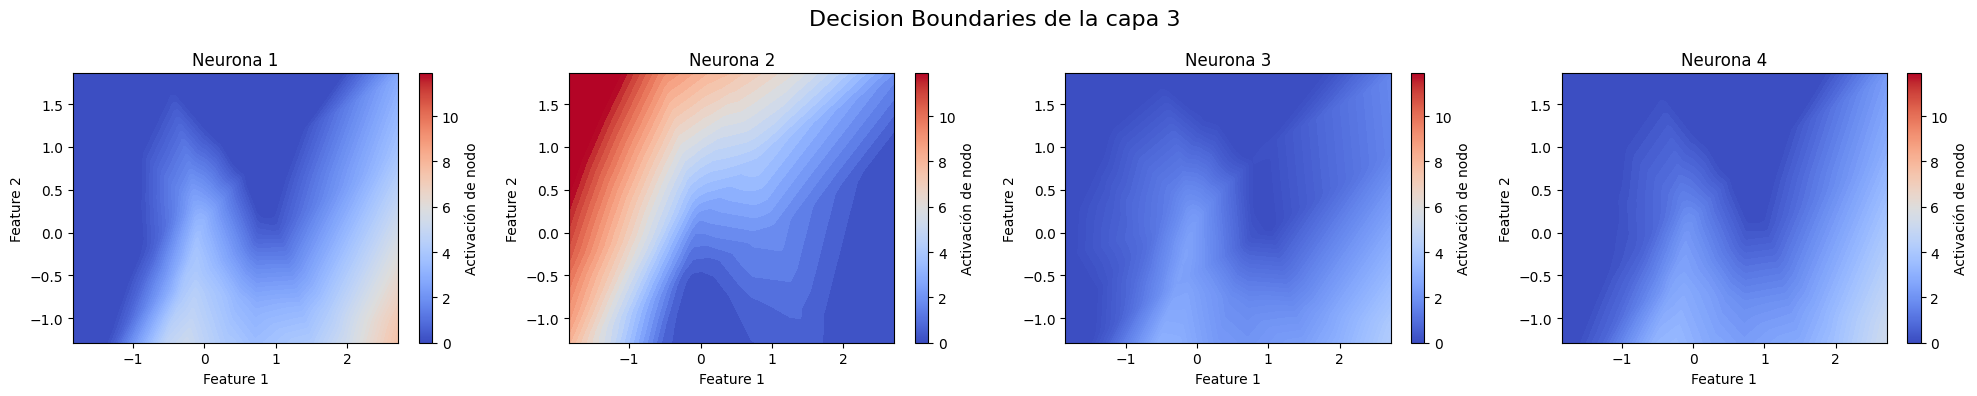
\includegraphics[width=1\linewidth]{images/plot_neuronas_L3.png}
  \caption{Límites de decisión de las neuronas de la tercera capa densa del modelo}
  \label{fig:sub1}
\end{figure}

\subsubsection{Capa de Salida (\texttt{output\_layer})}
La capa de salida tiene 2 neuronas y utiliza la función de activación Softmax. Esta capa genera dos valores de salida que representan las probabilidades de pertenecer a dos clases diferentes (por ejemplo, Clase A y Clase B). La función Softmax se define como
\[
\text{Softmax}(z_i) = \frac{e^{z_i}}{\sum_{j} e^{z_j}},
\]
lo que asegura que las salidas estén normalizadas, es decir, que la suma de las probabilidades sea igual a 1. Esta capa es utilizada para realizar la clasificación final.


\begin{figure}[H]
  \centering
  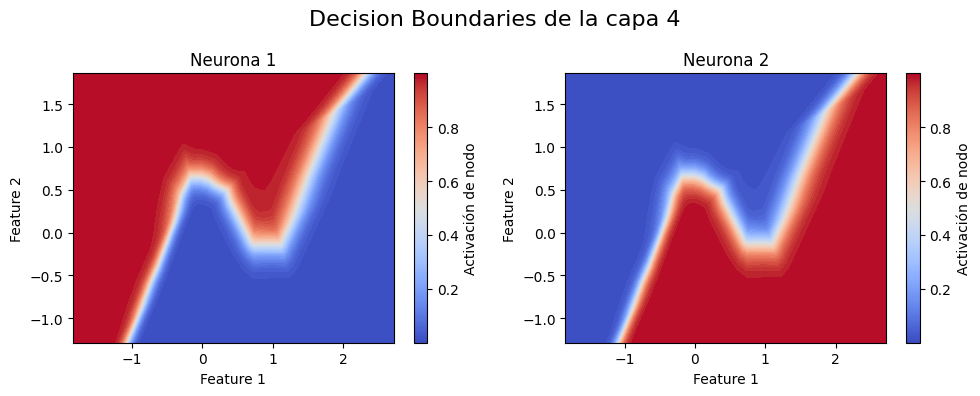
\includegraphics[width=1\linewidth]{images/plot_neuronas_L4.png}
  \caption{Límites de decisión de las neuronas de la cuarta capa densa del modelo}
  \label{fig:sub1}
\end{figure}

\subsubsection{Relación con los Gráficos}
Los gráficos que se presentan corresponden a los límites de decisión (\textit{decision boundaries}) aprendidos por las 8 neuronas de la segunda capa densa (\texttt{layer2}).

Cada gráfico representa la activación de una neurona específica en función de las dos características de entrada (\textit{Feature 1} y \textit{Feature 2}). 

Las zonas rojas indican activaciones altas, mientras que las zonas azules indican activaciones bajas o nulas. Neuronas con límites claros entre zonas (como las Neuronas 1, 3 y 4) están captando patrones relevantes en los datos. Por otro lado, neuronas como la Neurona 5, con una activación uniforme, podrían tener menor relevancia para el modelo.

\newpage
\appendix
\section*{Apéndice}
El código relacionado con este documento está disponible en el siguiente enlace de GitHub:
\begin{center}
    \href{https://github.com/angelleon01/aprendizaje_profundo}{github.com/angelleon01/aprendizaje\_profundo}
\end{center}

\end{document}
